\documentclass[12pt%
%,draft%
,xcolor=table
,aspectratio=169%
]{beamer}
%
\usepackage{fontspec}
\defaultfontfeatures{Ligatures=TeX}
%\setsansfont{Liberation Sans}
\usepackage{polyglossia}
\setdefaultlanguage{ngerman}
% Alternative template for talks of the Freie Universität Berlin.
% Created by Leonard R. König, <leonard.koenig@fu-berlin.de> following the
% guidelines on www.fu-berlin.de/cd
%
% (c) Leonard König, CC BY 4.0
%
% This template was written against UTF-8 capable LaTeX engines, specifically
% LuaLaTeX.

% Trying to get rather close to the ppt/odp template:
%  http://www.fu-berlin.de/sites/cd/downloads_container/PowerPoint_Praesentation_Anleitung.pdf

%%% font styles
\setbeamerfont{frametitle}{series=\bfseries}
\setbeamerfont{footline}{series=\bfseries}
\setbeamerfont{headline}{series=\bfseries}
\setbeamerfont{alerted text}{series=\bfseries}
%%%

% colordefs
\definecolor{fu_darkblue}{RGB}{0,51,102}
\definecolor{fu_seablue}{RGB}{0,102,204}
\definecolor{fu_lightblue}{RGB}{204,214,224}
\definecolor{fu_green}{RGB}{153,204,0}
\definecolor{fu_lightgrey}{RGB}{128,128,128}
\definecolor{fu_grey}{RGB}{95,95,95}
%
\definecolor{fu_red}{RGB}{204, 0, 0} % red text (used by \alert)
%%% end colordefs

%%% colors
\setbeamercolor*{title}{fg=fu_darkblue}
\setbeamercolor*{subtitle}{fg=fu_seablue}
\setbeamercolor*{frametitle}{fg=fu_darkblue}
\setbeamercolor*{footline}{fg=fu_grey,bg=fu_lightblue}
\setbeamercolor*{headline}{fg=fu_grey}

\setbeamercolor*{normal text}{fg=black}
\setbeamercolor*{alerted text}{fg=fu_red}
\setbeamercolor*{example text}{fg=fu_green}
\setbeamercolor*{structure}{fg=fu_darkblue}

\setbeamercolor*{block title}{fg=white,bg=black!50}
\setbeamercolor*{block title alerted}{fg=white,bg=black!50}
\setbeamercolor*{block title example}{fg=white,bg=black!50}

\setbeamercolor*{block body}{bg=black!10}
\setbeamercolor*{block body alerted}{bg=black!10}
\setbeamercolor*{block body example}{bg=black!10}

\setbeamercolor{bibliography entry author}{fg=fu_darkblue}

\setbeamercolor{item}{fg=fu_darkblue}
\setbeamercolor{navigation symbols}{fg=fu_lightgrey,bg=fu_grey}
%%% end colors

%%% title page
% Display logo (if exists) and right next to it, put our title + subtitle
\defbeamertemplate*{title page}{fu_titlepage}
{%
	\hskip .3\textheight
	\begin{minipage}[.4\textheight]{\textwidth}
		\begin{minipage}[.4\textheight]{0.25\textwidth}
			\inserttitlegraphic
		\end{minipage}%
		\begin{minipage}[.4\textheight]{0.75\textwidth}
			\begin{beamercolorbox}{title}
				\usebeamerfont{title}\inserttitle\par%
			\end{beamercolorbox}
			\vfill
			\ifx\insertsubtitle
				\@empty%
			\else
				\begin{beamercolorbox}{subtitle}
					\usebeamerfont{subtitle}\insertsubtitle\par
				\end{beamercolorbox}
			\fi
		\end{minipage}
	\end{minipage}%
	\hskip .3\textheight
}
%%% end title page

%%% headline
% display title, author and institute on the left;
% logo on the right.
\newcommand{\headlinetext}
{%
	\inserttitle\\[0.3em]%
	\insertauthor, %
	\insertshortinstitute
}
\newlength{\headlinewidth}
\setlength{\headlinewidth}{\paperwidth}
\addtolength{\headlinewidth}{-2\marginparsep}
\setbeamertemplate{headline}
{%
	\begin{beamercolorbox}[wd=\paperwidth]{headline}%
		\vskip5pt
		{\hspace*{\marginparsep}}%
		\parbox{.5\headlinewidth}
		{%
			\usebeamertemplate{title in head/foot}%
			\headlinetext%
		}%
		\begin{minipage}{.5\headlinewidth}%
			\hfill\usebeamertemplate*{logo}
		\end{minipage}%
		{\hspace*{\marginparsep}}%
	\end{beamercolorbox}%
}
%%% end headline

%%% footline
% title + date on the left, frame number on the right
\newcommand{\footlinetext}
{%
	\usebeamerfont{shorttitle}\insertshorttitle, %
	\usebeamerfont{shortdate}\insertshortdate
}
\setbeamertemplate{footline}
{%
	\begin{beamercolorbox}{footline}
		\vskip2pt
		\hspace{\marginparsep}%
		\footlinetext\hfill%
		\insertframenumber%
		\hspace{\marginparsep}
		\vskip2pt
	\end{beamercolorbox}%
}
%%% end footline

% don't use default templates for sidebars
\setbeamertemplate{sidebar right}{}
\setbeamertemplate{sidebar left}{}
\setbeamertemplate{title page}[fu_titlepage]
\usepackage{amsmath}
\usepackage{amsfonts}
\usepackage{amssymb}
\usepackage{graphicx}
\usepackage{algorithm}
\usepackage[noend]{algpseudocode}
%\usepackage{algorithmic}
\usepackage{tikz}
\usetikzlibrary{arrows,shapes,automata,petri,positioning,calc}
\usepackage{graphicx}
\usepackage{subfig}
\usepackage{pgfplots}
\usepackage{ stmaryrd }
\usepackage[normalem]{ulem}
\usepackage{circuitikz}
\usepackage{bohr}
\usepackage{csquotes}

\setbeamercolor{block title}{use=structure,fg=white,bg=structure.fg!75!black}
\setbeamercolor{block body}{parent=normal text,use=block title,bg=block title.bg!10!bg}


\usepackage{expl3}

\ExplSyntaxOn
\cs_new:Npn \displayasdecimal#1 {(#1) \sb {10}}
\cs_new:Npn \displayasoctal #1 {(\int_to_oct:n{#1}) \sb 8}
\cs_new:Npn \displayasbinary #1 {(\int_to_bin:n{#1}) \sb 2}
\ExplSyntaxOff

\newcounter{divline}
\def\rlwd{.5pt} \def\rlht{\dimexpr\dp\strutbox+\ht\strutbox} \def\rldp{.75ex}
\newcommand\mydiv[3][\relax]{%
  \ifx\relax#1\stepcounter{divline}\else\setcounter{divline}{#1}\fi%
  \mbox{}\hspace{\thedivline\dimexpr1ex}#2~\setbox0=\hbox{~$#3$}%
  \dumbstackengine{-\rlwd}{\rule[-\rldp]{\rlwd}{\rlht}~#3}{\rule{\dimexpr4pt+\wd0}{\rlwd}}%
}
\def\remainder#1{\stepcounter{divline}%
  \mbox{}\hspace{\dimexpr1ex+\thedivline\dimexpr1ex}~#1\setcounter{divline}{0}}
\makeatletter
\global\newlength\@stackedboxwidth
\newlength\@boxshift
\newsavebox\@addedbox
\newsavebox\@anchorbox
\newcommand*\dumbstackengine[3]{%
    \sbox{\@anchorbox}{$#2$}%
    \sbox{\@addedbox}{$#3$}%
    \setlength{\@stackedboxwidth}{\wd\@anchorbox}%
      \ifdim\wd\@addedbox>\@stackedboxwidth%
        \setlength{\@stackedboxwidth}{\wd\@addedbox}%
      \fi%
        \setlength{\@boxshift}{\dimexpr-\dp\@anchorbox -\ht\@addedbox -#1}%
        \usebox{\@anchorbox}%
        \hspace{-\wd\@anchorbox}%
        \raisebox{\@boxshift}{\usebox{\@addedbox}}%
        \hspace{-\wd\@addedbox}%
        \hspace{\@stackedboxwidth}%
}

\newcommand\decbin[9]{%
\par\smallskip
\makebox[3cm][r]{$#1$\ }\fbox{#2}\,\fbox{#3}\,\fbox{#4}\,\fbox{#5}\,\fbox{#6}\,\fbox{#7}\,\fbox{#8}\,\fbox{#9}\par}


\def\unsignedbytecalc#1{%
\par\smallskip
\noindent$#1_{10}$\par
\smallskip
\gdef\result{}%
$\left.\begin{array}{r@{\quad}|c}\udbc{#1}\end{array}\right\}\result$\par}

\def\udbc#1{%
\ifnum#1=\z@
\expandafter\@gobble
\else
\expandafter\@firstofone
\fi
{2)\!\underline{\,#1}&\edef\r{\ifodd#1 1\else 0\fi}\r\xdef\result{\r\result}\\
\expandafter\udbc\expandafter{\the\numexpr(\ifodd#1 #1-1\else#1\fi)/2\relax}%
}}


\author{Benjamin Tröster}
\title[Zahlendarstellung]{Zahlendarstellung}
\subtitle[IEEE-P 754-FLOATING-POINT-STANDARD]{IEEE-P 754-FLOATING-POINT-STANDARD}
%\pgfdeclareimage{titlegraphic}{../res/dwarf_logo2.png}
%\titlegraphic{\pgfuseimage{titlegraphic}}
%\date{}
%\subject{}
%
% FU settings
\institute[HTW Berlin]{Hochschule für Technik und Wirtschaft Berlin}
%\pgfdeclareimage[height=0.9cm]{logo}{../res/dwarf_logo}
%\logo{\pgfuseimage{logo}}
%
\usepackage[
backend=biber,
citestyle=alphabetic,bibstyle=authoryear
]{biblatex}
\addbibresource{sources.bib}


\begin{document}

\begin{frame}
\titlepage
\end{frame}

\begin{frame}{Fahrplan}
\tableofcontents[hideothersubsections]
\end{frame}

\section{IEEE-P 754}
\begin{frame}{IEEE-P 754}
\begin{itemize}
	\item Standardisierung von Gleitkommazahlen via IEEE Standard
	\item Original: \cite{IEEE754Original}
	\item Aktuell: \cite{cornea2009ieee}
	\item Schönes Paper: \cite{goldberg1991every}
\end{itemize}
\end{frame}

\subsection{Normierung (IEEE-Standard)}
\begin{frame}{Normierung (IEEE-Standard)}
\begin{itemize}
	\item In vielen Programmiersprachen lassen sich Gleitkomma-Zahlen mit verschiedener Genauigkeit darstellen
	\begin{itemize}
		\item C:
		\begin{itemize}
			\item float
			\item double
			\item long double
		\end{itemize}
		\item Java
		\begin{itemize}
			\item float
			\item double
		\end{itemize}
	\end{itemize}
	\item Der IEEE-Standard definiert mehrere Darstellungsformen
	\begin{itemize}
		\item IEEE single: 32 Bit
		\item IEEE double: 64 Bit
		\item IEEE extended: 80 Bit
	\end{itemize}
\end{itemize}
\end{frame}

\begin{frame}{IEEE-P 754-Floating-Point-Standard}
\begin{center}
	Maschinenformate des IEEE-Standards
\end{center}
\center
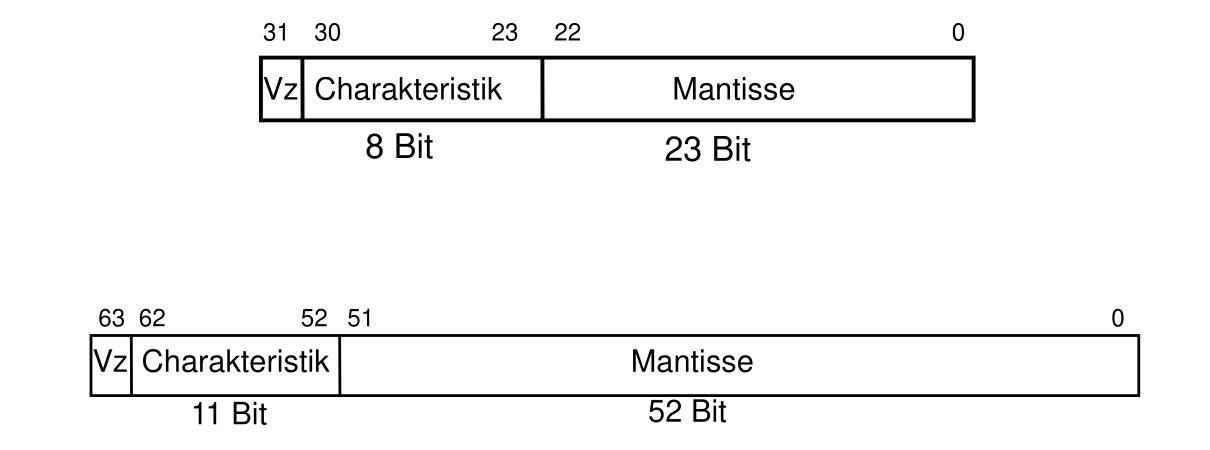
\includegraphics[scale=0.35]{pictures/ieee_machineformat}
\end{frame}

\begin{frame}{Eigenschaften des IEEE-P 754}
\begin{itemize}
	\item Die Basis $q$ ist gleich 2
	\item Das erste Bit der Mantisse wird implizit zu $1$ angenommen, wenn die Charakteristik nicht nur Nullen enthält
	\item \textcolor{red}{Normalisierung:} das erste Bit der Mantisse (die implizite $1$) steht vor dem Komma
	\item Ist die Charakteristik gleich 0, entspricht dies dem gleichen Exponenten wie die Charakteristik $1$
	\begin{itemize}
		\item Für die Darstellung der Subnormals und der Null
		\item Normalisierte Zahlen kommen nur bis Minreal: Werte kleiner Darstellbar, aber nicht normalisiert
	\end{itemize}
	\item Das erste Bit der Mantisse wird aber dann explizit dargestellt
	\item \textcolor{red}{Auch die Null ist darstellbar}
\end{itemize}
\end{frame}

\begin{frame}{Eigenschaften des IEEE-P 754}
\begin{itemize}
	\item Sind alle Bits der Charakteristik gleich 1, signalisiert dies eine Ausnahmesituation
	\item Wenn zusätzlich die Mantisse gleich Null ist, wird die Situation \enquote{overflow} (bzw. die \enquote{Zahl} $\pm \infty$) kodiert
	\item Dies erlaubt es dem Prozessor, eine Fehlerbehandlung einzuleiten
	\item Intern arbeiten Rechner nach dem IEEE-Standard mit 80 Bit, um Rundungsfehler unwahrscheinlicher zu machen
	\item Charakteristik gleich 1 und Mantisse ungleich 0: NaN
\end{itemize}
\end{frame}

\begin{frame}{Zusammenfassung der Parameter des IEEE-P 754}
\begin{table}[]
\begin{tabular}{|c|c|c|}
\hline
\rowcolor[HTML]{656565} 
{\color[HTML]{333333} \textbf{Parameter}} & {\color[HTML]{333333} \textbf{Single}} & {\color[HTML]{333333} \textbf{Double}} \\ \hline
Bits Gesamt 			& 32 			& 64		\\ \hline
Bits Mantisse          & 23(+1) 		& 52(+1)    \\ \hline
Bits Charakteristik    & 8				& 11        \\ \hline
Exponent Bias  			&  +127			& +1023     \\ \hline
$E_{max}$ 				& +127       	& +1023 	\\ \hline
$E_{min}$ 				&  -126      	& -1022 	\\ \hline
\end{tabular}
\end{table}
Der Bias ist $2^{n-1}-1$ anstatt $2^{n-1}$
\end{frame}

\begin{frame}{Zusammenfassung des 64-Bit-IEEE-Formats}
\begin{table}[]
\begin{tabular}{|c|c|c|}
\hline
\rowcolor[HTML]{656565} 
{\color[HTML]{333333} \textbf{Charakter.}} & {\color[HTML]{333333} \textbf{Zahlenwert}} & {\color[HTML]{333333} \textbf{Bemerkung}} \\ \hline
$0$ 			& $(-1)^{Vz} 0,Mantisse \cdot 2^{-1022}$ 		& Subnormalisiert	\\ \hline
$1$ 			& $(-1)^{Vz} 1,Mantisse \cdot 2^{-1022}$  		&  Normalisiert   	\\ \hline
$\ldots$		& $(-1)^{Vz} 1,Mantisse \cdot 2^{-1023}$ 		&    Normalisiert 	\\ \hline
$2046$			& $(-1)^{Vz} 1,Mantisse \cdot 2^{1023}$		&	Normalisiert	\\ \hline
$2047$ 			& $Mantisse = 0 : (-1)^{Vz} \infty$     		& Overflow 	\\ \hline
$2047$ 			& $Mantisse \neq 0 :$					 		& $NaN$ 	\\ \hline
\end{tabular}
\end{table}
\end{frame}
\section{Beispiele}

\begin{frame}{Beispiel: $4,4_{10}$}
Übersicht: Umrechnung $4,4_{10} \to X_2$
\begin{itemize}
	\item Vorgehen via Horner-Schema:
	\begin{itemize}
		\item Ganzzahliger Teil: $4_{10} = 100_2$
		\item Nachkommateil: $0,4 = 0, \overline{0110}_2$
	\end{itemize}
	\item Normalisierung: $100, \overline{0110}_2 \cdot 2^0 = 1,00 \overline{0110}_2 \cdot 2^2$
	\item Verrechnen mit Bias: $2$ Bits Shifted: $127+4 = 129$
	\item Charakteristik: $129_{10} = 010000001_2$
	\item $01000000100\overline{0110}_2 = 01000000100011001100110011001100_2 \approx 4,3999996185302734375$
\end{itemize}
\end{frame}

\begin{frame}{Umrechnung: Ganzzahliger \& Nachkommateil}
\begin{columns}[T] % align columns
\begin{column}{.6\textwidth}
\vspace*{-1.cm}
\begin{center}
Ganzzahliger Anteil
\begin{table}[]
\begin{tabular}{ccc}
 & Div & Mod (Remainder) \\
$4 : 2$ & $2$ & 0 \\
$2 : 2$ & $1$ & 0 \\
$1 : 2$ & $0$ & 1 \\ 
\end{tabular}
\end{table}
\end{center}
\end{column}%
\hfill%
\begin{column}{.4\textwidth}
\vspace*{-.75cm}
\begin{center}
Nachkommabereich
\begin{table}[]
\begin{tabular}{lll}
 &  & Carry \\
$0,4 \cdot 2$ & $0,8$ & 0 \\
$0,8 \cdot 2$ & $1,6$ & 1 \\
$0,6 \cdot 2$ & $1,2$ & 1 \\
$0,2 \cdot 2$ & $0,4$ & 0 \\
$0,4 \cdot 2$ & $\ldots$ & 
\end{tabular}
\end{table}
\end{center}
\end{column}%
\end{columns}
\end{frame}

\begin{frame}{Zusammensetzen und Verrechnung mit Bias}
\begin{itemize}
	\item  Normalisierung: $100, \overline{0110}_2 \cdot 2^0 = 1,00 \overline{0110}_2 \cdot 2^2$
	\begin{itemize}
		\item Verschiebung um zwei Bits
		\item $1$ vor dem Komma redundant
	\end{itemize}
	\item Bias: 8 Bit $2^7-1$, $B = 011111111_2 = 127_{10}$
	 -127 -> d.h. Zahlen beginnen nicht bei 0, sonder bei -127
	\begin{itemize}
		\item Um die Zahlen ohne Zweierkomplement darstellen zu können
	\end{itemize}
	\item Einrechnen des Offsets: Daher $127 + 2 = 129$ ist der codierte Exponent	
	\item $129_{10} = 10000001_2$ ist das Exponent
	\item $10000001_2$ $1,00011001100110011001100_2$
	\item Mantisse $1$ vor dem Komma kann weg
	\item $0100000010001100110011001100110_2 = 408ccccc_{16}$
\end{itemize}
\end{frame}

\begin{frame}{Float (32 Bit) Minreal, Maxreal, Smallreal}
\begin{itemize}
	\item Maxreal: $3.402823 \cdot 10^{38} = 340282300000000000000000000000000000000$
	\begin{itemize}
		\item $01111111011111111111111111111101_2$
		\item Expoent: $2^127$ mit Bias: $254_{10} = 111111101_2$
	\end{itemize}
	\item Minreal: $1.175494 \cdot 10^{-38} = 0.0000000000000000000000000117549393043$
	\begin{itemize}
		\item $00000000011111111111111111111101_2$
		\item Exponent: $2^{-126}$ mit Bias: 0, Mantisse voll besetzt
	\end{itemize}
	\item Smallreal: $1.0000001$ als Addition von $1.0 + 1.0_2 \cdot 2^{-22}$
	\begin{itemize}
		\item Binär: $1_{10} = 00111111100000000000000000000000_2$
		\item Kleinster Wert der mit +1 darstellbar ist: $1 \cdot 10^{-7} = 00110011110101101011111110010101_2$
		\item Addition ergibt aufgrund des Exponenten der 1: $00111111100000000000000000000001$
		\item \textcolor{red}{Gegenbeispiel: $1.00000001_{10} = 00111111100000000000000000000000$}
		\item Fehlerrate: $-1E-8 = -1 \cdot 10^{-8}$
	\end{itemize}
\end{itemize}
\end{frame}

\section{Rundung}
\begin{frame}{Rundung}
\begin{itemize}
	\item IEEE Standard Forderung:
	\begin{itemize}
		\item Das Ergebnis, das man durch eine arithmetische Operation mit dem Rechner erhält, soll dasselbe sein, als wenn man exakt rechnet und anschließend entsprechend eines geeigneten Modus rundet
	\end{itemize}
	\item IEEE Standard definiert vier Rundungsmodi:
	\begin{itemize}
		\item Rundung zum nächstliegenden Gleitkommawert:
		\begin{itemize}
			\item Falls der Abstand zu zwei Gleitkommawerten gleich ist, wird zu jenem Wert gerundet, dessen
niederwertigste Stelle eine gerade Ziffer ist (\enquote{round-to-even}-Regel)
		\end{itemize}
		\item Rundung zum nächsten Gleitkommawert in Richtung $0$
		\item Rundung zum nächsten Gleitkommawert in Richtung $+ \infty$
		\item Rundung zum nächsten Gleitkommawert in Richtung $- \infty$
	\end{itemize}
\end{itemize}
\end{frame}

\begin{frame}{Rundungen}
\begin{figure}
\center
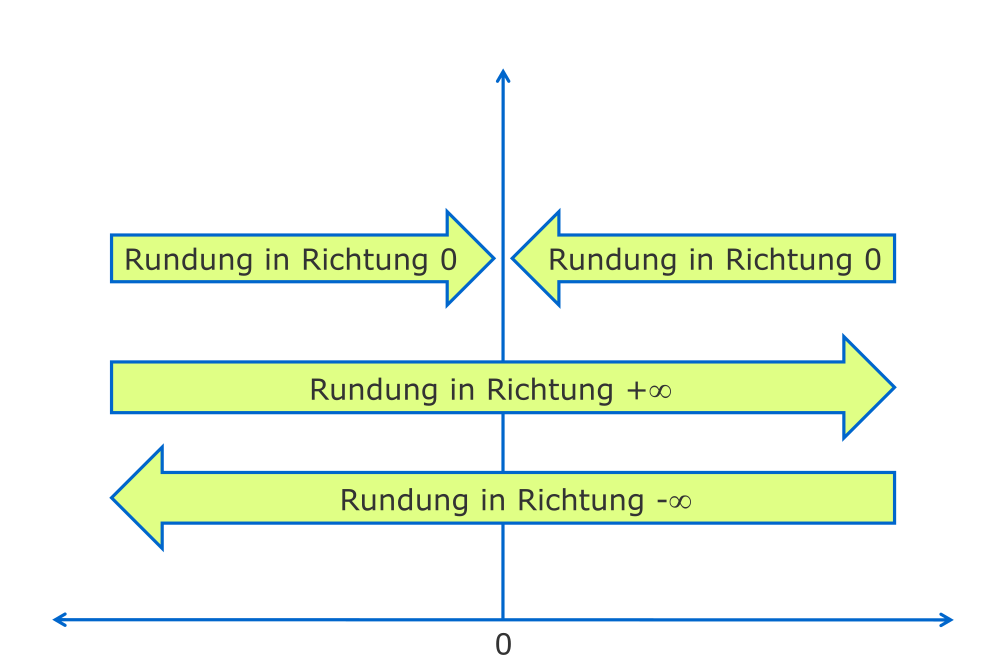
\includegraphics[scale=0.325]{pictures/rundung1}
\end{figure}
\end{frame}

\begin{frame}{Rundungen}
\begin{itemize}
	\item Am schwierigsten zu implementierende Rundung:
	\begin{itemize}
		\item Rundung zum nächstliegenden Gleitkommawert
	\end{itemize}
	\item Eine Möglichkeit: Summe exakt berechnen und anschließend runden
	\begin{itemize}
		\item sehr lange Register, sehr aufwändig
	\end{itemize}
	\item Auch mit weniger Hardware-Aufwand möglich?
	\item Es gibt zwei Fälle für eine Rundung bei Addition und Subtraktion:
	\begin{itemize}
		\item auftretender Übertrag
		\item Exponentenanpassung
	\end{itemize}
\end{itemize}
\end{frame}

\begin{frame}{Beispiel a: Übertrag bei Addition}
Basis 10, drei signifikante Stellen (d.h. Mantisse hat maximal drei Stellen)
\begin{align*}
	& &2,34 	& \cdot 10^2\\
	& &+8,51	& \cdot 10^2\\ \cline{3-4}
	& &10,85 	& \cdot 10^2 \\
	& & & 	\\
	&\text{wird gerundet zu } & 1,08 	& \cdot 10^3
\end{align*}
\end{frame}

\begin{frame}{Beispiel b: ungleiche Exponenten}
Basis 10, drei signifikante Stellen
\begin{align*}
	2,34 	& \cdot 10^2 & 	2,34 	& \cdot 10^2\\
	+2,56	& \cdot 10^0 & 0,0256 	& \cdot 10^2	\\ \cline{3-4}
	& & 2,3656 & \cdot 10^2\\
	& & &\\
	&\text{wird gerundet zu} & 2,37 & \cdot 10^2
\end{align*}
\end{frame}

\begin{frame}{Beispiel c: Übertrag und ungl. Exponenten}
Basis 10, drei signifikante Stellen
\begin{align*}
	& \text{beides} & 9,51 & \cdot 10^2 \\
	& 				&  +0,642 & \cdot 10^2 \\ \cline{3-4}
	&				& 10,152 & \cdot 10^2 \\
	& \text{wird gerundet zu} & 1,02 & \cdot 10^3
\end{align*}
\end{frame}

\begin{frame}{Problem}
\begin{itemize}
	\item Für jeden dieser Fälle muss die Summe mit mehr als drei signifikanten Stellen berechnet werden, um eine korrekte Rundung zu ermöglichen
	\item Es gibt auch Fälle, bei denen eine Rechnung mit mehr als drei signifikanten Stellen notwendig ist, obwohl keine Rundung erfolgt 
	\begin{itemize}
		\item Subtraktion nahe beieinanderliegender Zahlen
		\item Siehe Beispiel d
	\end{itemize}		
\end{itemize}
\end{frame}

\begin{frame}{Beispiel d: Subtraktion von naheliegenden Zahlen}
\begin{align*}
& & 1,47 & \cdot 10^2 \\
& &-0,876 & \cdot 10^2 \\ \cline{3-4}
& & 0,594 & \cdot 10^2
\end{align*}
\begin{itemize}
	\item Bei den bisherigen Beispielen reichte eine zusätzliche Stelle aus
	\item Es gibt aber auch Fälle, bei denen dies nicht genügt
\end{itemize}
\end{frame}

\begin{frame}{Beispiel e}
\begin{align*}
& & 1,01 & \cdot 10^2 \\
& & -0,0376 & \cdot 10^2 \\ \cline{3-4}
& & 0,9724 & \cdot 10^2 \\
& & & \\
& \text{wird gerundet zu} & 0,972 & \cdot 10^2
\end{align*}
\begin{itemize}
	\item Wenn die niederwertigste Ziffer $6$ von $0,0376$ gestrichen würde, wäre das Ergebnis $0,973$ anstatt $0,972$
\end{itemize}
\end{frame}

\subsection{Rundungs- und Prüfstelle}

\begin{frame}{Rundungs- und Prüfstelle}
\begin{itemize}
	\item Es lässt sich zeigen, dass unter Vernachlässigung der \enquote{round-to-even}-Regel zwei weitere Stellen für eine korrekte Rundung stets ausreichend sind
	\item Diese beiden Stellen heißen:
	\begin{itemize}
		\item die Rundungsstelle $r$ und
		\begin{itemize}
			\item Falls $r > 0$ ist Runden einfach, da wir nicht in der Mitte sind
			\item Was wenn $r=0$?
		\end{itemize}
		\item Prüfstelle $g$
		\begin{itemize}
			\item Sagt, ob wir $r$ genauer betrachten müssen, wir könnten in der Mitte ($g=5_{10}$) sein
		\end{itemize}
	\end{itemize}
	\item Aber: Die \enquote{round-to-even}-Regel erfordert zusätzlichen Aufwand.
\end{itemize}
\end{frame}

\begin{frame}{Beispiel f:}
Fünf signifikante Stellen:
\begin{align*}
	& 4,5674 \cdot 10^0 & & ~~~~4,5674 \\
	& 2,5001 \cdot 10^{-4} & & +0,00025001 \\ \cline{4-5} 
	& & & 4,56765001\\
	& & & ~~~~~~~~~gr \\
	& \text{wird gerundet zu} & & 4,5677
\end{align*}
\begin{itemize}
	\item Rundungsstelle $r$ und Prüfstelle $g$ genügen nicht
	\item Information: sind alle niederwertigeren Stellen hinter der Rundungsstelle gleich Null, dann nur ein \textcolor{red}{sticky}-Bit
\end{itemize}
\end{frame}

\subsection{Sticky-Bit}

\begin{frame}{Sticky-Bit}
\begin{itemize}
	\item Für eine richtige Rundung ist die Information ausreichend, ob alle niederwertigeren Stellen hinter der Rundungsstelle gleich Null sind
	\item Es genügt ein Bit: \enquote{sticky}-Bit
	\item Wenn eine der Stellen, die durch das Angleichen der Exponenten beider Operanden gestrichen werden, ungleich Null ist, wird das \enquote{sticky}-Bit gesetzt
	\item Falls das Ergebnis in gleichem Abstand zum oberen und unteren nächstliegenden Fließkommawert liegt, entscheidet das "sticky"-Bit, ob nach oben oder nach unten gerundet wird
\end{itemize}
\end{frame}


\section*{Quellen}
\appendix
\begin{frame}[allowframebreaks]
  \frametitle<presentation>{Quellen}
\printbibliography
\end{frame}
\end{document}